\documentclass{tufte-book}

%!TEX TS-program = pdflatex
%!TEX encoding = UTF-8

\hypersetup{colorlinks}% uncomment this line if you prefer colored hyperlinks (e.g., for onscreen viewing)

%%
% Book metadata
\title{Tools for Learning}
\author[Rod Allrich]{Rod Allrich}
\publisher{Typeset by Kautilya Chenna}


%%
% If they're installed, use Bergamo and Chantilly from www.fontsite.com.
% They're clones of Bembo and Gill Sans, respectively.
%\IfFileExists{bergamo.sty}{\usepackage[osf]{bergamo}}{}% Bembo
%\IfFileExists{chantill.sty}{\usepackage{chantill}}{}% Gill Sans

%\usepackage{microtype}

%%
% Just some sample text
\usepackage{lipsum}

%%
% For nicely typeset tabular material
\usepackage{booktabs}

%%
% For graphics / images
\usepackage{graphicx}
\setkeys{Gin}{width=\linewidth,totalheight=\textheight,keepaspectratio}
\graphicspath{{graphics/}}

% The fancyvrb package lets us customize the formatting of verbatim
% environments.  We use a slightly smaller font.
\usepackage{fancyvrb}
\fvset{fontsize=\normalsize}

%%
% Prints argument within hanging parentheses (i.e., parentheses that take
% up no horizontal space).  Useful in tabular environments.
\newcommand{\hangp}[1]{\makebox[0pt][r]{(}#1\makebox[0pt][l]{)}}

%%
% Prints an asterisk that takes up no horizontal space.
% Useful in tabular environments.
\newcommand{\hangstar}{\makebox[0pt][l]{*}}

%%
% Prints a trailing space in a smart way.
\usepackage{xspace}

%%
% Some shortcuts for Tufte's book titles.  The lowercase commands will
% produce the initials of the book title in italics.  The all-caps commands
% will print out the full title of the book in italics.
\newcommand{\vdqi}{\textit{VDQI}\xspace}
\newcommand{\ei}{\textit{EI}\xspace}
\newcommand{\ve}{\textit{VE}\xspace}
\newcommand{\be}{\textit{BE}\xspace}
\newcommand{\VDQI}{\textit{The Visual Display of Quantitative Information}\xspace}
\newcommand{\EI}{\textit{Envisioning Information}\xspace}
\newcommand{\VE}{\textit{Visual Explanations}\xspace}
\newcommand{\BE}{\textit{Beautiful Evidence}\xspace}

\newcommand{\TL}{Tufte-\LaTeX\xspace}

% Prints the month name (e.g., January) and the year (e.g., 2008)
\newcommand{\monthyear}{%
	\ifcase\month\or January\or February\or March\or April\or May\or June\or
	July\or August\or September\or October\or November\or
	December\fi\space\number\year
}


% Prints an epigraph and speaker in sans serif, all-caps type.
\newcommand{\openepigraph}[2]{%
	%\sffamily\fontsize{14}{16}\selectfont
	\begin{fullwidth}
		\sffamily\large
		\begin{doublespace}
			\noindent\allcaps{#1}\\% epigraph
			\noindent\allcaps{#2}% author
		\end{doublespace}
	\end{fullwidth}
}

% Inserts a blank page
\newcommand{\blankpage}{\newpage\hbox{}\thispagestyle{empty}\newpage}

\usepackage{units}

% Typesets the font size, leading, and measure in the form of 10/12x26 pc.
\newcommand{\measure}[3]{#1/#2$\times$\unit[#3]{pc}}

% Macros for typesetting the documentation
\newcommand{\hlred}[1]{\textcolor{Maroon}{#1}}% prints in red
\newcommand{\hangleft}[1]{\makebox[0pt][r]{#1}}
\newcommand{\hairsp}{\hspace{1pt}}% hair space
\newcommand{\hquad}{\hskip0.5em\relax}% half quad space
\newcommand{\TODO}{\textcolor{red}{\bf TODO!}\xspace}
\newcommand{\na}{\quad--}% used in tables for N/A cells
\providecommand{\XeLaTeX}{X\lower.5ex\hbox{\kern-0.15em\reflectbox{E}}\kern-0.1em\LaTeX}
\newcommand{\tXeLaTeX}{\XeLaTeX\index{XeLaTeX@\protect\XeLaTeX}}
% \index{\texttt{\textbackslash xyz}@\hangleft{\texttt{\textbackslash}}\texttt{xyz}}
\newcommand{\tuftebs}{\symbol{'134}}% a backslash in tt type in OT1/T1
\newcommand{\doccmdnoindex}[2][]{\texttt{\tuftebs#2}}% command name -- adds backslash automatically (and doesn't add cmd to the index)
\newcommand{\doccmddef}[2][]{%
	\hlred{\texttt{\tuftebs#2}}\label{cmd:#2}%
	\ifthenelse{\isempty{#1}}%
	{% add the command to the index
		\index{#2 command@\protect\hangleft{\texttt{\tuftebs}}\texttt{#2}}% command name
	}%
	{% add the command and package to the index
		\index{#2 command@\protect\hangleft{\texttt{\tuftebs}}\texttt{#2} (\texttt{#1} package)}% command name
		\index{#1 package@\texttt{#1} package}\index{packages!#1@\texttt{#1}}% package name
	}%
}% command name -- adds backslash automatically
\newcommand{\doccmd}[2][]{%
	\texttt{\tuftebs#2}%
	\ifthenelse{\isempty{#1}}%
	{% add the command to the index
		\index{#2 command@\protect\hangleft{\texttt{\tuftebs}}\texttt{#2}}% command name
	}%
	{% add the command and package to the index
		\index{#2 command@\protect\hangleft{\texttt{\tuftebs}}\texttt{#2} (\texttt{#1} package)}% command name
		\index{#1 package@\texttt{#1} package}\index{packages!#1@\texttt{#1}}% package name
	}%
}% command name -- adds backslash automatically
\newcommand{\docopt}[1]{\ensuremath{\langle}\textrm{\textit{#1}}\ensuremath{\rangle}}% optional command argument
\newcommand{\docarg}[1]{\textrm{\textit{#1}}}% (required) command argument
\newenvironment{docspec}{\begin{quotation}\ttfamily\parskip0pt\parindent0pt\ignorespaces}{\end{quotation}}% command specification environment
\newcommand{\docenv}[1]{\texttt{#1}\index{#1 environment@\texttt{#1} environment}\index{environments!#1@\texttt{#1}}}% environment name
\newcommand{\docenvdef}[1]{\hlred{\texttt{#1}}\label{env:#1}\index{#1 environment@\texttt{#1} environment}\index{environments!#1@\texttt{#1}}}% environment name
\newcommand{\docpkg}[1]{\texttt{#1}\index{#1 package@\texttt{#1} package}\index{packages!#1@\texttt{#1}}}% package name
\newcommand{\doccls}[1]{\texttt{#1}}% document class name
\newcommand{\docclsopt}[1]{\texttt{#1}\index{#1 class option@\texttt{#1} class option}\index{class options!#1@\texttt{#1}}}% document class option name
\newcommand{\docclsoptdef}[1]{\hlred{\texttt{#1}}\label{clsopt:#1}\index{#1 class option@\texttt{#1} class option}\index{class options!#1@\texttt{#1}}}% document class option name defined
\newcommand{\docmsg}[2]{\bigskip\begin{fullwidth}\noindent\ttfamily#1\end{fullwidth}\medskip\par\noindent#2}
\newcommand{\docfilehook}[2]{\texttt{#1}\index{file hooks!#2}\index{#1@\texttt{#1}}}
\newcommand{\doccounter}[1]{\texttt{#1}\index{#1 counter@\texttt{#1} counter}}

% Generates the index
\usepackage{makeidx}
%\makeindex

\begin{document}
	
	% Front matter
	\frontmatter
	
	% r.1 blank page
	% \blankpage
	
	% r.3 full title page
	\maketitle
	
	% v.4 copyright page
	\newpage
	\begin{fullwidth}
		~\vfill
		\thispagestyle{empty}
		\setlength{\parindent}{0pt}
		\setlength{\parskip}{\baselineskip}
		Copyright \copyright\ \the\year\ \thanklessauthor
		
		\par\smallcaps{\thanklesspublisher}
		\par\textit{First printing, \monthyear}
	\end{fullwidth}

	% r.5 contents
	\tableofcontents
	
	\listoffigures
	
	\listoftables
	
	\chapter{Active Learning}

This is a very wide and deep topic that I will only attempt to summarize here. The gist of the matter is this - \textbf{Learners Should Be Active}. Anything a learner can do to be actively involved in the subject at hand is the best plan of attack. The \textbf{best non-example} is this: Go to a lecture in one of your courses and sit passively all hour, then leave. This is the exact opposite of active learning. It could well be called passive learning. You just sit and listen, and perhaps take verbatim notes (writing down exactly what the instructor places on the overhead or blackboard). Couldn't a robot do that?


\marginnote{
I believe the Chinese have a saying that goes something like this:

\textit{Hear and Forget,}

\textit{See and Remember,}

\textit{Do and Understand.}}

Active learning is ``doing'' and this leads to understanding.

The \textbf{best example} of active learning is this: Go deliver a lecture. That requires a lot of preparation and understanding of the material. And after its all done, the subject is well understood by the individual who delivered the lecture (the audience may or may not have connected at all with what was said-in fact, a great lecture can be delivered to an empty room!). In most college classrooms however, the one (the student, the learner) who should be the most active is, in fact, the least active. It's kind of absurd that the one who knows the material best (the instructor) is the most active in our classrooms. This goes against the principle of active learning. Below I have listed some things that a student can do to promote active learning in and out of the classroom.


\section{Suggestions}

\begin{itemize}
	\item Don't take verbatim notes in a lecture course. As you actively listen in lecture, construct a set of notes that mean something to you. This may involve making drawings of material presented as text on the overhead. It may involve incomplete items that you will fill in after class after you have consulted the textbook or talked with the instructor. It may involve Mind Maps (see the book by Tony Buzan).
	
	\item Ask more questions in class!! Most students appear trained to come into a classroom and passively sit all hour. Break the mold. Ask questions that will help you make sense of the lecture material. Not only are you helping yourself, but also some other student who probably wanted to ask the same question. Questions from students who have kept up with the material (and attend class) are a valuable asset to the instructor because it is important feedback that lets the instructor know what was perhaps missed by students (or what needs further explanation). Questions from students who frequently miss class (or don't study) are a pain in the rear because their questions don't reflect the state of learning of the entire class. Be a good learner and your questions will automatically be good.
	
	\item Seek out other sources of the course material. Don't just rely on what the instructor gives you. Go find other texts, talk to other instructors, find references in the library, search the Internet, etc. Some of the material you find will be better than what is presented in your class.
	
	\item Study with a partner and take turns orally presenting topics to each other (with and without your notes as help).
	
	\item Create possible quiz/test questions and exchange them with someone in class who also made up questions.
	
	\item Place terms and their definitions on opposite sides of index cards for later review/self-quizzing.
	
	\item Obtain old quizzes/exams and try to answer them without any help.
\end{itemize}

	\chapter{Attention}

When a student lacks attention during any class period (or wherever they are when studying/learning), that student is not efficiently learning the material at hand. Without attention, the information cannot be funneled to the brain's learning center. The figure below illustrates the critical role of attention (and motivation) in the learning process.

\begin{marginfigure}%
	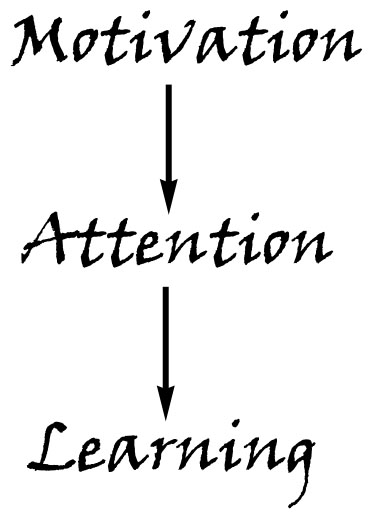
\includegraphics[width=0.75\linewidth]{./images/attention}
	\label{fig:attention}
\end{marginfigure}

This figure starts with motivation. A student must be motivated (intrinsically and/or extrinsically) in order to have attention in class. Motivation is best fueled by an intrinsic source. A student with intrinsic motivation would say ``I like this stuff and its fun to learn''. A student with only extrinsic motivation might say ``This is a required class for me so I'm just doing the minimum so I can graduate''. A student with no motivation would be chatting with a neighbor during class or working a crossword puzzle. Whatever the source, \textbf{motivation leads to attention}. In other words, motivation is a prerequisite to attention. You can't have prolonged attention without motivation. Think of attention as a focus on the material to be learned.

\textbf{Attention leads to learning}. In other words, attention is a prerequisite to learning. And there's no way around it! If a student pays little attention in class, very little learning will occur at that time. I estimate that if a student has good attention in class, it is worth 2-3 hours of study out of class. In other words, \textbf{pay attention in class and it reduces your study time outside of class}.

A student cannot pay attention in class if he/she is sleepy or ill. A good night's sleep will allow the student to be at maximum efficiency  in the classroom. Sleep and health often go together. A lack of sleep makes a person more susceptible to illness. When a student is ill, focus in class is almost impossible. It is also impossible to chat with a neighbor in class and at the same time pay attention to the instructor (or whomever is speaking).

This idea/notion of paying attention in class is one I see many student fail at. I can't tell you how many inattentive students I see each day-it would take too long for me to report.

	\chapter{Distributed Practice}

Distributed practice is a technique whereby the student distributes his/her study effort in a given course over many study sessions that are relatively short in duration. This can be compared to massed practice (otherwise known as cramming) whereby the student conducts few but long study sessions for a given course. It has been proved beyond a shadow of a doubt that meaningful learning is promoted when distributed practice is conducted. In contrast, massed practice promotes rote learning. For the long-term benefit of the student, distributed practice should be the method an excellent student chooses to use. After a 4-5 year college career, a student who followed the distributed practice technique would be miles ahead of a student who followed the massed practice technique. Unfortunately, some college courses encourage massed practice by giving only 2-3 exams during the semester (and little else for assessment). When only 2-3 exams are given, the student masses study sessions immediately prior to each exam. This testing frequency (2-3 exams/semester) also promotes, the less desirable, rote learning.

How can a student implement distributed practice? Well, it takes motivation and determination to get this all rolling. Probably one good way is to schedule study times on a week to week basis at the beginning of each semester. That is, set aside one 50 minute study session each day for each course. Do this for Monday through Saturday, leaving Sunday as an off-day or catch-up day or even as a total relaxation day or family day. After the semester gets rolling, adjustments may need to be done. Perhaps some courses don't need the daily 50 minute study session M-Sat. with some sessions skipped during the week. In other cases, some courses may require more than one daily study session. Only the individual student can judge whether adjustments are needed. If a student needs so much study time that there isn't enough time in the day to schedule sessions, that student should consider dropping a course or two.

For distributed practice to be successful, the student must be able to follow his/her study schedule. \textbf{Don't let interruptions spoil it}. Think of your study schedule as a work schedule, something that must be followed. If you find that other people/other activities prevent you from keeping on schedule, then you are going to falter. Go hide someplace during your study sessions (the library works good for this if you find a corner up in the stacks). Another hint, take study breaks- study for 50 minutes then get up for a 5-10 minute break. Then come back to more of the same subject, or better yet, go on to a new subject. Another hint- try not to take two similar courses during the same semester. Sometimes when a student takes two similar courses, material from one class may interfere with the ability to learn material in the other class. This isn't always the case, but in general it is better to take courses (in any one semester) that are distinct from each other.
	\chapter{Elaboration}

The principle of elaboration is this: Whatever you are studying in a course, try to expand (elaborate) upon what you are given. For example, if the instructor gives you 5 functions of the liver during a lecture, go out and try to find information about more functions (that the instructor didn't mention or perhaps doesn't know). In the end, you may add two more functions of the liver and in the process remember all of them better. For another example, if your assigned textbook discusses three theories of personality, try to find other theories in library books, other references, or even from talking to instructors other than your own. Don't limit yourself to what any one instructor (or textbook) tells you. They all have their biases which can prevent you from seeing (and learning) all the facts. When you elaborate, you end up understanding the information better and it will therefore be easier to recall and use.

So in summary, elaboration is a process whereby the learner expands upon the information given to them during a lecture, lab, reading assignment, etc. It's an act of empowerment, and puts the ultimate control of what is learned into the learner's hands. Right where the power should be in the first place! If a student were to practice the elaboration principle over a long period of time (and over many courses), he or she would surely ``look different'' to any potential employer or interviewer when a job was being sought out. This student would have a richer bank of information to call upon during the interview process (compared to other students). The other students with the same degree would ``look'' very similar to each other because they took mostly the same courses and received all the same information (because they didn't go out and elaborate). So set yourself apart (by learning more than the herd average) and the effort will be well rewarded.
	\chapter{Generation Effect}

The Generation Effect refers to the fact that you will remember something better if you are involved in its creation or can create it after study. For example, in a course you may see the below table in a textbook or handout. During your study sessions you would usually look over the table and note its content. However, that is not all that should be done. You should attempt to reproduce the table from scratch. That is, can you reproduce the table starting with a blank sheet of paper? When you attempt that, it will be clear that you don't know the information in the table as well as your thought. When you study like this, you will remember so much more about the table information. 

\begin{table}[h]
	\begin{center}
		\footnotesize%
		\begin{tabular}{cc}
			\toprule
			Age of Bull (months) & Testes weight (g) \\
			\midrule
			2 & 20 \\
			12 & 370 \\
			36 & 590 \\
			\bottomrule
		\end{tabular}
	\end{center}
	\caption{Age of Bull vs Testes weight.}
	\label{tab:bull}
\end{table}

This same principle applies to figures and any text material. During study periods, you should attempt to reproduce important figures or terms from scratch. Take the word acetylcholine, for example. The best method to help learn its spelling is to write it down on paper and pronounce it. Take the word apart: acetyl-cho-line. Define it: acetylcholine is a neurotransmitter. Work with the word several times over several days. Then try to generate it.

It's one thing to say you know something, but until you can draw it (or speak it) without looking at the originial, you may well be fooling yourself. That leads to a good question-Who is on the U.S. quarter (coin) and which way is he facing? You probably will guess (although you have handled a quarter many times), but if you have drawn the coin several times you would remember better.
	\chapter{Goals are Golden}

Setting goals is a very helpful technique that students can implement at any time. Setting goals and then reaching them can be, psychologically, very uplifting. It feels good to reach a goal. But there's also a danger. Not reaching a goal can be a downer or outright depressing. So be careful! Start with small, easy goals and then build them up to stretch your ability.

Here are some rules for setting goals. 

Goals should be \textbf{S. M. A. R. T.}

\textbf{S}pecific goals are the best. Good example of this: Read pages 12-21 in physics (chapter 1) tonight starting at 7pm. Here's the bad version: Read in my physics book sometime today.

\textbf{M}easurable goals are good. Good example of this: Read 20 pages in my chemistry book by noon today. Here's the bad version: Read some pages in my chemistry book this week.

\textbf{A}ttainable goals work best. Good example of this: Attend every class session this week and work at my job at Smitty's a total of 8 hours this week. Here's the bad version: Attend every class session this week and work 30 hours this week at my job at Smitty's and work 20 hours at Hooters.

\textbf{R}ealistic goals should be proposed. Good example of this: Since I want to improve my GPA (now standing at 1.81) I will try to get B's or better in all my classes. Here's the bad version: Since I want to improve my GPA (now standing at 1.81) I will try to get A's in all my classes.

\textbf{T}imely goals help. Good example of this: I am going to read 2 chapters in my biology book by noon tomorrow. Here's the bad version: I am going to read all my assigned reading in biology by the time of exam \#1 (which is scheduled 3 weeks from today).
	\chapter{Meaningful Learning}

Meaningful learning refers to the concept that the learned knowledge (lets say a fact) is fully understood by the individual and that the individual knows how that specific fact relates to other stored facts (stored in your brain that is). For understanding this concept, it is good to contrast \textbf{meaningful learning} with the much less desirable, \textbf{rote learning}.

Rote learning is where you memorize something without full understanding and you don't know how the new information relates to your other stored knowledge. For our example, lets say we learn 5 facts in a math course during a full semester by rote learning. This can be illustrated by the figure below. The 5 facts (labeled 1-5) are stored in memory as separate items although in real life they are related to each other. When the student rote learned these facts, the brain stored them as distinct, unrelated knowledge that can only be recalled individually (one fact at a time). When this student recalls one fact the other 4 facts are not recalled (or activated) at that moment. In other words, thinking about fact \#5 does not lead the student to think about facts \#1-4. Contrast that to the below discussion on recall after meaningful learning.

\begin{figure}
	\centering
	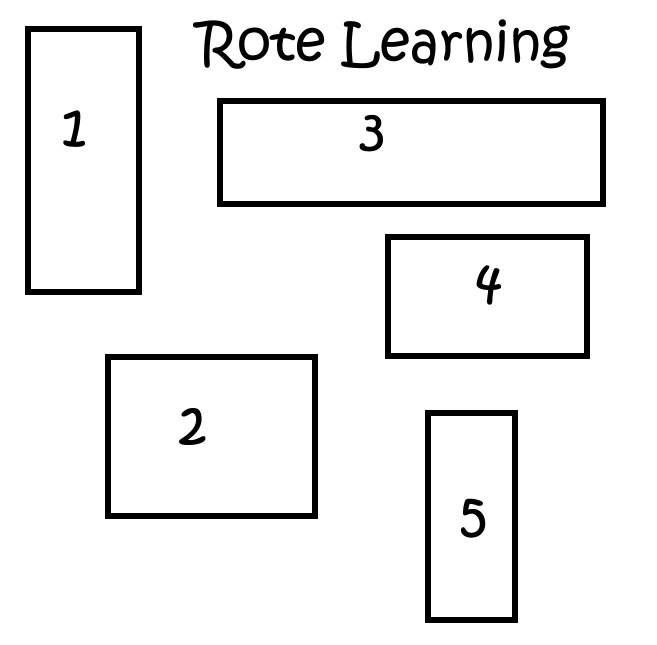
\includegraphics[width=0.55\linewidth]{./images/mean1}
	\caption{Rote Learning}
	\label{fig:mean1}
\end{figure}

When meaningful learning occurs (using our example of 5 math facts) the facts are stored in a relational manner (see figure below). That is, the brain stores them together because they are related to each other. Now, when one fact is recalled, the other facts are also recalled at that moment (or shortly thereafter). In other words, recalling fact \#5 activates the memory for facts \#2 and \#4, and this in turn leads to recalling facts \#1 and \#3. This phenomenon is called the spread of activation. This is the gist of meaningful learning. Problem-solving for this student would be easier than for the student who rote learned the same 5 facts.  Which one of these students would you like to hire for your company? Some suggestions on how to ensure meaningful learning appear below the figure. 

\begin{figure}
	\centering
	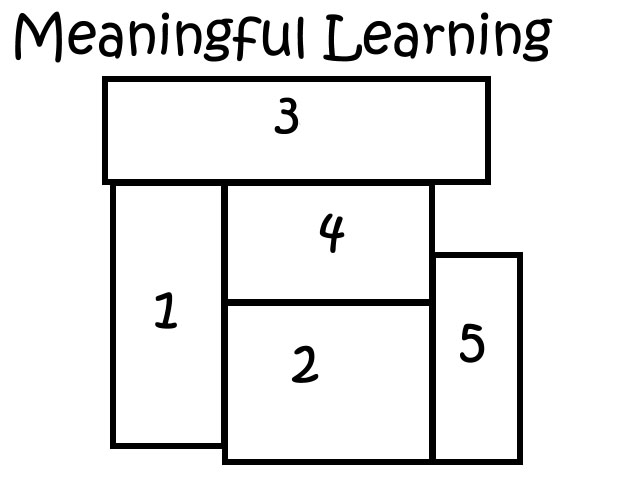
\includegraphics[width=0.55\linewidth]{./images/mean2}
	\caption{Meaningful Learning}
	\label{fig:mean2}
\end{figure}

\section{Suggestions}

\begin{itemize}
	\item Make sure what you learn is in your proximal zone.
	\item If in doubt, ask the instructor how some new knowledge is related to other course material.
	\item Have a study partner ask you questions that require recall of related material.
	\item Make a figure that illustrates what you should know about a specific topic and its related material.
\end{itemize}
	\chapter{Practice Retrieval}

Retrieval is a process of recalling what we have in memory. So, for our purposes, recall and retrieval refer to the same process. When we take tests or quizzes (or other such instruments), our minds attempt to recall answers (or relevant information that can be used to formulate an answer) to the questions we read.  Hopefully, we have previously stored this information in our brain (as a result of studying and learning) and can now recall it and write down the answer. To answer the questions then, we must recall the relevant information. Taking a test involves retrieval. Usually, our performance on a test is recorded and counts toward our final course grade.

\textbf{Practice Retrieval} refers to the fact that students should practice their retrieval skills prior to the test (or quiz or whatever). Wouldn't it be better to practice first, then take the real test?? Most people would answer yes. The figure below illustrates my concept of retrieval. Its really like getting information off of a diskette. [Putting information on the diskette (like saving a file) is called encoding when we refer to our memory. Encoding occurs during learning (hopefully).] Suggestions on how to perform practice retrieval are listed below the figure.

\begin{figure}
	\centering
	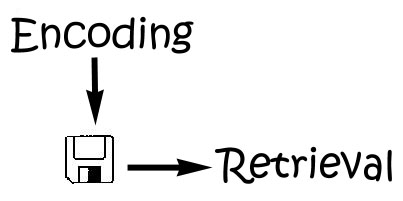
\includegraphics[width=0.55\linewidth]{./images/practice}
	\caption{Encoding and Retrieval}
	\label{fig:practice}
\end{figure}

\section{Suggestions}

\begin{itemize}
	\item Have a fellow student ask you questions as she reads her notes or looks in the textbook.
	\item Have a fellow student write down questions on a sheet of paper that you will answer later.
	\item Attempt to answer questions from old quizzes/tests.
	\item Visit Web sites of similar courses (to the one your in) and attempt to answer questions you find there.
\end{itemize}
	\chapter[Preview-View-Review]{Preview-View-Review System of Study}

This technique can be applied in many ways during the learning process. The View in this case refers to either a lecture, book chapter, lab handout, or anything to be studied. Most of us go to the lecture, read the chapter or lab handout without preparing our mind for what is to come during the lecture or reading. What would be best is to prepare our mind for the upcoming material. This is where the Preview comes in handy. The purpose of the Preview is to let our minds get a flavor of what is to come before the actual event occurs. In other words, preview the material before we study (or listen/take notes in the case of a lecture). During the process of Preview, our mind will automatically activate related knowledge it has stored on the subject. For example, if we were going to read a chapter on kidney function, the Preview would activate related knowledge and make it more likely that we would remember things during the View (for example, the actual reading of the chapter).

So, what actually is the Preview? Well, it can be many different things. Lets say we are about to read the chapter on kidney function. One technique (for a Preview) would be to skim the chapter reading bold text, looking at figures and tables, and reading questions/summary statements at the end of the chapter. This process would give us a flavor of things to come during the full reading of the chapter. Cognitive psychologists would call the Preview an advanced organizer. It is well known that if you preview something, you are more likely to remember it after the study session. In other words, you are more likely to store it in memory by attaching it to items previously learned. One other example: If you are going to a lecture on kidney function, a good Preview would be to discuss kidney function with a fellow student before getting to class. Between the two of you, many related topics would have been brought up and discussed before the lecture started. In this manner, your mind would have opened the file entitled ``kidneys'' and you would be prepared to put more items into the file during lecture.

Now, what about the Review part of this. The Review refers to a process of refreshing your mind of what has been encountered during the View. The Review is exactly how it sounds, to review. Much has been written on reviewing and I suggest you search the cognitive psychology literature for this information. Briefly, there is an art to reviewing. First, material should be reviewed more than a total of one time. Some would suggest the first Review  take place shortly after the View has occurred (within one hour). Then, the next (second) Review should take place one day after the View. The third Review should then occur one week after the original View. Now, depending upon the material, subsequent reviews would take place on a weekly to monthly basis. Any given Review should be short, say 5-10 minutes. The objective is to scan the material, activating memories as you go along.

In summary, this technique can be applied to almost any situation. Probably, for a beginner in this area, the first step to take is to practice previewing material. Obviously, discipline and motivation are required for success. Good Luck.
	\chapter{Zone of Proximal Development}

This is an important concept to understand because it can guide you to what you should learn next about a topic. At this given moment, we all have certain knowledge stored in our memories about specific topics. For example, I have a memory bank labeled "hepatic physiology" somewhere in my brain that contains what I know about liver physiology. This is my Present Knowledge on the topic. Since I don't know everything about liver physiology, there are still ideas/facts/concepts that I can learn and add to my memory bank. However, of all the stuff I can still learn (and there's a lot), a subset of it would be best (and easier) to learn next and other subsets would be best left alone until later. That subset that would be best (and easier) to learn next is contained in the Proximal Zone. The subsets that should be left until later are contained within the Distal Zone.

As learning proceeds, a portion of the Proximal Zone becomes part of the Present Knowledge, and as a consequence, a smaller Proximal Zone remains. Notice in the figure below how the \#1 Proximal Zone was incorporated into the present knowledge after learning occurred. Hence, over time, Present Knowledge grows but there is always a Proximal Zone present (albeit, ever changing). Also, there is always a Distal Zone present that represents knowledge to be learned later. If you knew everything there was to know about a subject, there would be no Proximal or Distal Zones (fat chance that will ever happen). Suggestions on how to involve the Zone of Proximal Development concept in your learning are listed at the very end of this page. 

\begin{figure}
	\centering
	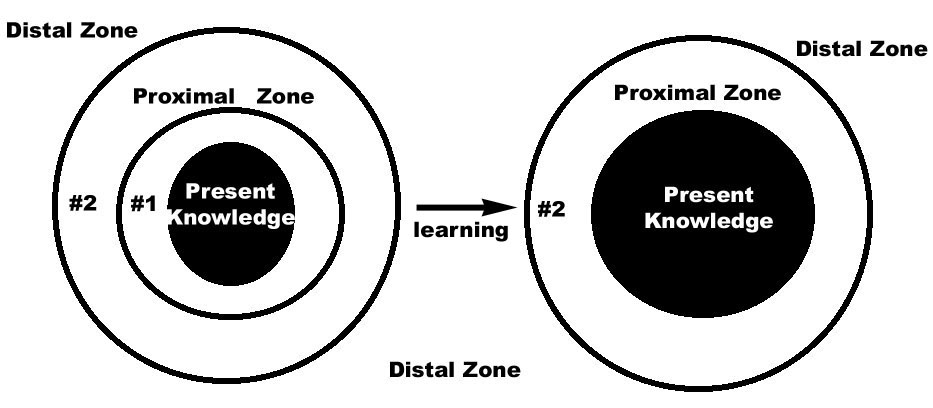
\includegraphics[width=0.80\linewidth]{./images/pz}
	\caption{Proximal Zone}
	\label{fig:pz}
\end{figure}

The take home message of this concept is that at any given time for any student (young or old), there exists material that would be the next best material to learn. For example, some courses are offered in specific sequences (i.e. Biology 101, Biology 102, etc.) and it is best to enroll in, and finish, Biology 101 before going onto Biology 102. The hard part of all of this is knowing where we stand and what we should learn next (in a given subject area). A good instructor will be able to help individual students determine if they are prepared for that instructor's course. One sad note-just because a student has completed a given course (perhaps a prerequisite) doesn't mean that the student is prepared to more forward to other subsequent courses (in a series, for example). Why? Because not every student comes out of a course learning what should have been learned (even if they passed the course). This all snowballs for some students and they find themselves in courses where they cannot learn the material because they don't have a large enough Present Knowledge structure. One last comment: The above figure also illustrates the fact that new knowledge (the material learned from the Proximal Zone) is always attached to Present Knowledge. This leads to the principle-The more you know, the easier it is to learn more (in terms of the figures, the larger the solid circle, the more area is available to attach additional knowledge). These last comments refer to Meaningful Learning and not to Rote Learning.

\section{Suggestions}

\begin{itemize}
	\item Be honest with yourself. Don't proceed to the next course in a series if you didn't learn what you should have learned in the first course. If you proceed, in this case, you will learn less from the subsequent course or courses. In the long-term, it will be like building a house on a weak foundation-sooner or later things won't work out (failure to succeed, dead-end jobs, etc.).
	\item Seek help from your instructors. See if they can determine if you are ready for their course or subsequent courses. Have them suggest corrective measures if deficiencies are noted.
	\item Make a resolution to ``learn how to learn''. It's a life-long task. 
\end{itemize}
	
	\printindex

\end{document}